\section{Introduction}
This chapter presents the results of the statistical analysis and interprets the findings in relation to the research objectives. It also compares the results with previous studies and provides a critical discussion.

\section{Descriptive Statistics}
Begin by presenting basic summaries of your data:
\begin{itemize}
    \item Summary measures such as mean, median, standard deviation
    \item Distribution of variables (possibly shown via histograms or box plots)
\end{itemize}

\begin{table}[H]
    \centering
    \caption{Descriptive Statistics of Key Variables}
    \begin{tabular}{lccc} \hline
        \textbf{Variable} & \textbf{Mean} & \textbf{Std. Dev.} & \textbf{N} \\ \hline
        X1 & 12.5 & 3.2 & 100 \\
        X2 & 9.8 & 2.1 & 100 \\ \hline
    \end{tabular}
    \label{tab:desc}
\end{table}

\section{Model Estimation Results}
Present the key outcomes of your model. For example, regression results:

\begin{table}[H]
    \centering
    \caption{Regression Estimates}
    \begin{tabular}{lcc} \hline
        \textbf{Variable} & \textbf{Coefficient} & \textbf{p-value} \\ \hline
        Intercept & 2.45 & 0.001 \\
        X1 & 0.78 & 0.021 \\
        X2 & -0.34 & 0.105 \\ \hline
    \end{tabular}
    \label{tab:regression}
\end{table}

\section{Model Diagnostics}
Include plots and tests to check the validity of your model:
\begin{itemize}
    \item Residual plots
    \item Tests for normality and homoscedasticity
    \item R-squared or adjusted R-squared
\end{itemize}

\begin{figure}[H]
    \centering
    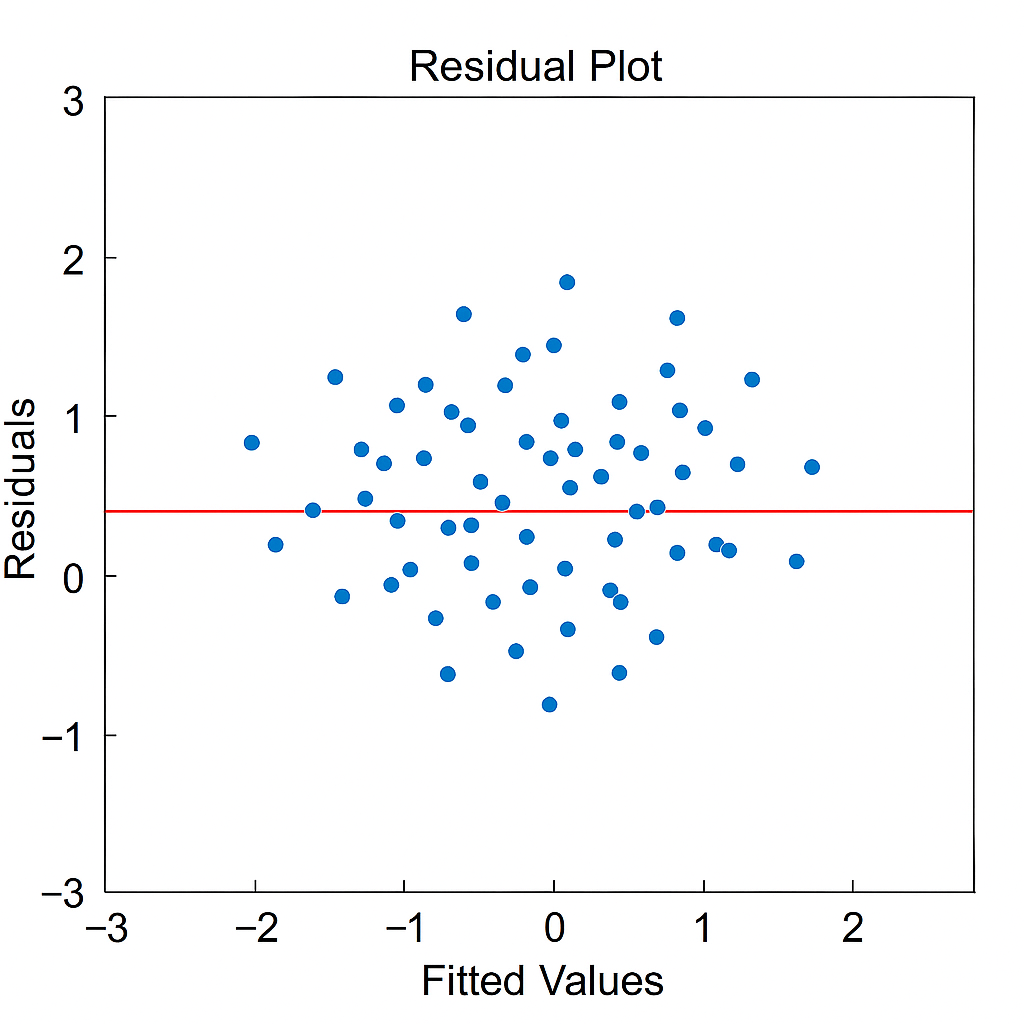
\includegraphics[width=4in]{residuals.png}
    \caption{Residual Plot of the Fitted Model}
    \label{fig:residuals}
\end{figure}

\section{Interpretation of Results}
Discuss the significance and implications of your results:
\begin{itemize}
    \item Interpret the direction and magnitude of the coefficients.
    \item Explain which variables are statistically significant.
    \item Relate findings back to your hypotheses or research questions.
\end{itemize}

\section{Comparison with Previous Studies}
Compare your findings with existing literature:
\begin{itemize}
    \item Are your findings consistent with previous studies? Cite relevant works.
    \item Highlight any contradictions or new insights.
\end{itemize}

For example, the positive effect of X1 is in line with the results reported by \cite{Si86}, while the insignificant impact of X2 contrasts with the findings in \cite{Het16}.

\section{Summary}
Summarize the key findings presented in this chapter. Mention any interesting patterns or unexpected outcomes that require further investigation.
